\chapter{Networking Hardwares}

Networking hardware or networking equipment typically refers to devices facilitating the use of a computer network. 
Typically, this includes gateways, routers, network bridges, switches, hubs, and repeaters. 
Computer networking devices are also called network equipment, Intermediate Systems (IS) or InterWorking Unit (IWU).
Units which are the last receiver or generate data are called hosts or data terminal equipment.
The most common kind of networking hardware today is copper-based Ethernet adapters, helped largely by its standard inclusion on most modern computer systems.

\section{Gateway}
A gateway is a network point that acts as an entrance to another network.
A gateway may contain devices such as protocol translators, impedance matching devices, rate converters, fault isolators, or signal translators as necessary to provide system interoperability. 
It also requires the establishment of mutually acceptable administrative procedures between both networks.
A protocol translation/mapping gateway interconnects networks with different network protocol technologies by performing the required protocol conversions.
While forwarding an IP packet to another network, the gateway might or might not perform Network Address Translation.
\section{Router}
A router is a device that forwards data packets between computer networks, creating an overlay internetwork. A router is connected to two or more data lines from different networks. When a data packet comes in one of the lines, the router reads the address information in the packet to determine its ultimate destination. Then, using information in its routing table or routing policy, it directs the packet to the next network on its journey. Routers perform the "traffic directing" functions on the Internet. 
When multiple routers are used in interconnected networks, the routers exchange information about destination addresses, using a dynamic routing protocol. Each router builds up a table listing the preferred routes between any two systems on the interconnected networks. A router has interfaces for different physical types of network connections, (such as copper cables, fiber optic, or wireless transmission).
\section{Bridge}
A network bridge is a network device that connects more than one network segment. In the OSI model bridging acts in the first two layers.
There are four types of network-bridging technologies: simple bridging; multiport bridging; learning, or transparent bridging; and source route bridging.
Network bridges work similarly to network switches, but the traffic is managed differently. A bridge will only send traffic from one side to the other if it is going to a destination on the other side. This is different to a layer 1 switch which sends all traffic from either side. Sometimes network bridges are called layer 2 switches.
Since they need to look at the contents of the traffic going into them, they are much more complicated than a hub or repeater
\section{Switch}
A network switch is a computer networking device that links network segments or network devices. The term commonly refers to a multi-port network bridge that processes and routes data at the data link layer (layer 2) of the OSI model. Switches receives a message from any device connected to it and then transmits the message only to the device for which the message was meant. This makes the switch a more intelligent device than a hub (which receives a message and then transmits it to all the other devices on its network). 
Switches may operate at one or more layers of the OSI model, including data link and network. A device that operates simultaneously at more than one of these layers is known as a multilayer switch.
\begin{figure}[htbp]
\begin{center}
	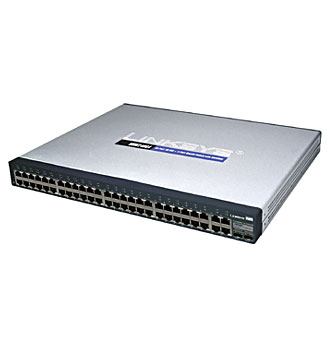
\includegraphics[width=5cm]{./Networking/ntwhardware/switch.jpg}
\caption{Switch}
\label{default}
\end{center}
\end{figure}

\section{Hubs}
An Ethernet hub or hub is a device for connecting multiple Ethernet devices together and making them act as a single network segment. It has multiple input/output (I/O) ports, in which a signal introduced at the input of any port appears at the output of every port except the original incoming. A hub works at the physical layer (layer 1) of the OSI model.
 A hub does not examine or manage any of the traffic that comes through it: any packet entering any port is rebroadcast on all other ports.
 It is barely aware of frames or packets and mostly operates on raw bits or symbols. Consequently, due to the larger collision domains, packet collisions are more frequent in networks connected using hubs than in networks connected using more sophisticated devices.
 Hubs are classified as physical layer devices in the OSI model. At the physical layer, hubs support little in the way of sophisticated networking. Hubs do not read any of the data passing through them and are not aware of their source or destination addressing. A hub simply receives incoming Ethernet frames, regenerates the electrical signal on the bit (more precisely the symbol) level, and broadcasts these symbols out to all other devices on the network.
 \begin{figure}[htbp]
\begin{center}
	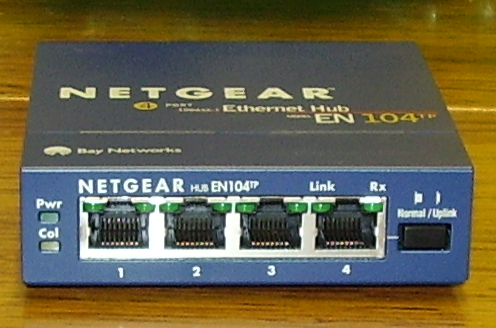
\includegraphics[width=5cm]{./Networking/ntwhardware/hub.jpg}
\caption{Network Hub}
\label{default}
\end{center}
\end{figure}

\section{Repeaters}
A repeater is an electronic device that receives a signal and retransmits it at a higher level or higher power, or onto the other side of an obstruction, so that the signal can cover longer distances.
In telecommunication,repeater can be ann analog device that amplifies an input signal regardless of its nature (analog or digital) or a digital device that amplifies, reshapes, retimes, or performs a combination of any of these functions on a digital input signal for retransmission.
In computer networking, because repeaters work with the actual physical signal, and do not attempt to interpret the data being transmitted, they operate on the physical layer, the first layer of the OSI model.
Repeaters are used to boost signals in coaxial and twisted pair cable and in optical fiber lines. An electrical signal in a cable gets weaker the further it travels, due to energy dissipated in conductor resistance and dielectric losses. Similarly a light signal traveling through an optical fiber suffers attenuation due to scattering and absorption. In long cable runs, repeaters are used to periodically regenerate and strengthen the signal.

